\section{Question 3}

``Draw the class diagrams for all the hierarchies in your source code. Explain why you created these
hierarchies and classify their type (e.g., “Is-a” and “Polymorphism”). Considering the lectures, are
there hierarchies that should be removed? Explain and implement any necessary change.''
\\

\begin{figure}[h]
\centering
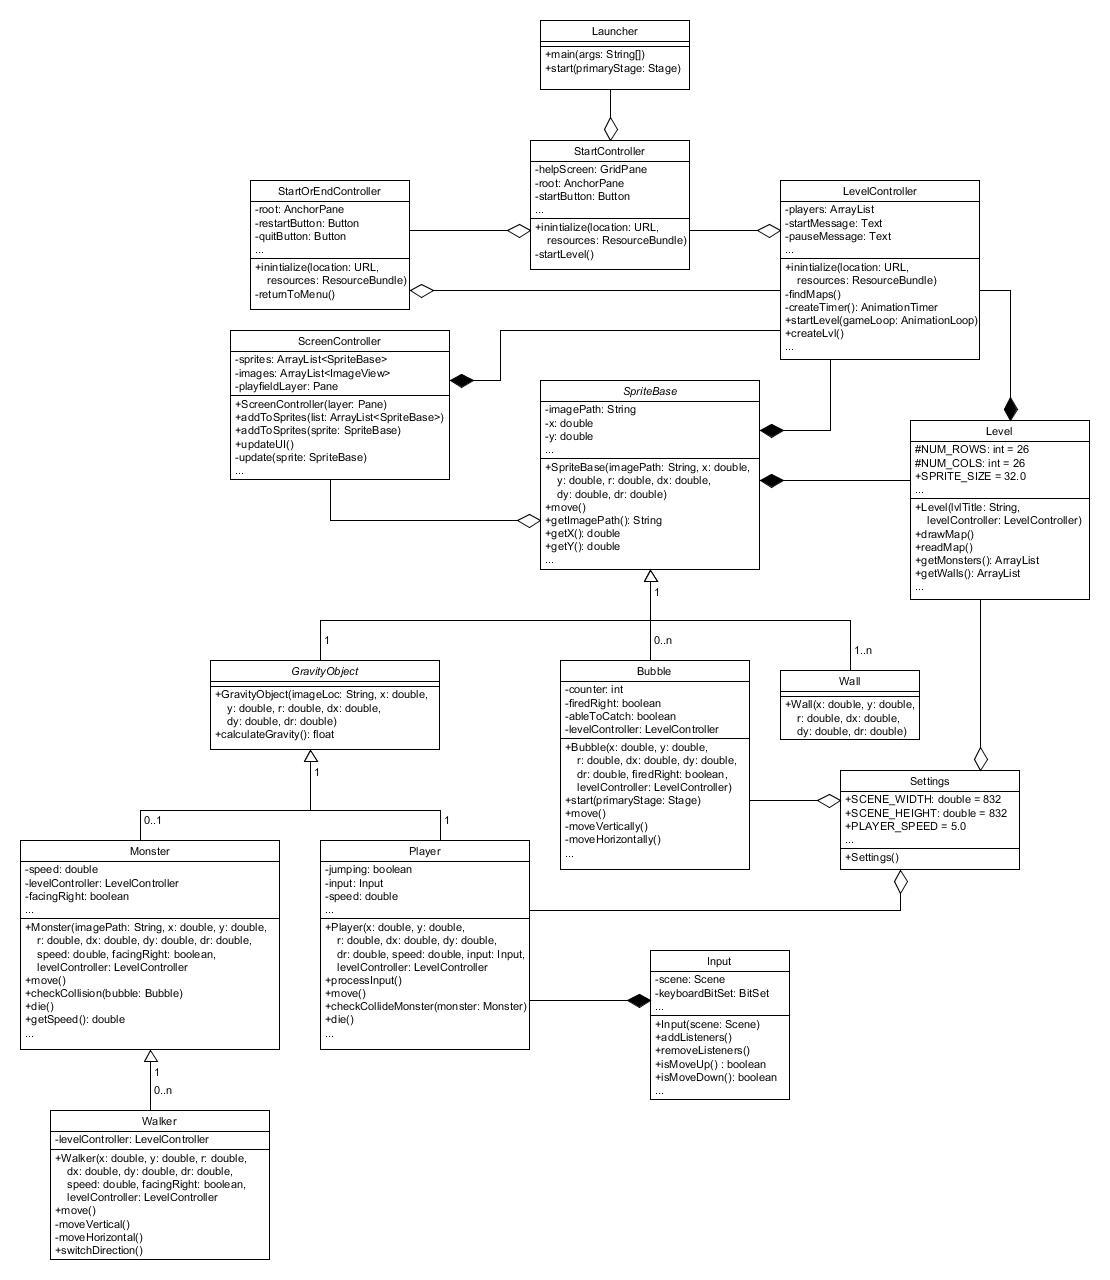
\includegraphics[width=\textwidth]{classDiagramsUML_3.jpg}
\caption{The class diagram for the whole project.}
\end{figure}

\noindent The hierarchies that can be seen in the class diagram in figure 2.1, have been chosen to stop the code from becoming too complex, and to allow both the programmers and developers, as well as anyone who would be looking at the code to have a better understanding of how the code is set up. The hierarchies were also created in this way, to insure that no class would get too long.
\\\\
\noindent The following hierarchies can be seen in the class diagram:
\begin{itemize}
\itemsep0em 
\item There is Polymorphism between SpriteBase (the super class) and its three sub classes GravityObject, Bubble and Wall.
\item There is Polymorphism between GravityObject (the super class) and its two sub classes Monster and Player.
\item There is Is-a between Monster (the super class) and its sub class Walker.\\
\end{itemize} 

\noindent The hierarchies work well because they aren't too complex and because they allow each of the components of the game to be created without having to rewrite code multiple times.     